\documentclass{IEEEtran}

\usepackage{graphicx}
\graphicspath{ {./images/} }
\usepackage{caption}
\usepackage{subcaption}

\begin{document}

\title{Automated Conversion of Sketches into Source Game Engine Maps}
\author{Cameron Stevenson}
 
 \maketitle
 
\begin{abstract}
abstract...
\end{abstract}

\section{Introduction}

Video games made by Valve run on the Source game engine, and share a common map editor and map file specification. Counter Strike: Global Offensive (CS:GO) is one such game, which has many past and present community-made maps for the competitive game mode. The map editor operates in 3D and is more suited to blocking in finer details. Blocking in the basic layout of the map can be time consuming, especially with complex geometry such as curves. If the process of taking a 2D layout idea and making a 3D map from it were automated, it would free up creative potential for map authors. This paper aims to automatically interpret sketched layouts to create the geometry and entities necessary to have a compilable and playable map.

\section{Background}
\subsection{Text Detection and Recognition}
Rosebrock \cite{rosebrock2018opencv} and others detail a method of detecting text bounding boxes with EAST, and recognising words with Tesseract. EAST is capable of detecting word and line text in natural backgrounds \cite{zhou2017east}. Tesseract \cite{smith2007overview} is Google's text recognition engine which maintains uncertainty throughout the letter recognition process until words are recognised. Feeding the bounding boxes found by EAST into Tesseract is usually a robust method of recognising font text in real images.

Methods exist for recognising handwritten characters from different people. Pal et al. \cite{pal2010handwritten} skeletonize characters and use neural networks to recognise characters. This method operates on images of single characters.

General shape similarity methods may be applied, such as those found in Skiena's book \cite{skiena2020algorithm} Hamming distance of two shapes is how much area they don't overlap in when placed on top of each other. Hausdorff distance focusses on the place where 2 shapes differ the most, measuring the furthest distance you can be from one shape if you lie on any point in the other shape. Skeleton comparison reduces shapes to their core structure, then compares topology and length/angle features.

\subsection{Sketch Interpretation}

Naya et al. \cite{naya2002direct} recognise the need for allowing users to sketch designs before converting them into computer models. Their proposal shows how sketched lines can be interpreted within certain tolerances to give digital representations. 

Similarly Zargar et al. \cite{zargar2019introducing} interpret perspective sketches to generate 3D models.

Yetiş et al. \cite{yetics2019auto} observe that freeform sketches generally rely on human experience to resolve ambiguities when interpreting their meaning. Also, discontinuities and irregularity in lines can cause imprecise models. They attempt to use deep learning in the 2D to 3D conversion, and it gets the basic outline of architectural sketches correct.

\subsection{Polygon Simplifcation}

The Douglas-Peucker algorithm \cite{douglas1973algorithms} for polygon simplification is additive. It begins with 2 points of the original polygon, and adds other points from the original polygon which are sufficiently far from the current approximation. Once every non-added point is sufficiently close to the approximation, it terminates.

\subsection{Polygon Triangulation}
Asano et al. \cite{asano1986polygon} demonstrate how collinearity of vertices can be used to minimise triangle count beyond n-2, at the cost of time complexity. Triangulation cannot be faster than sorting. 

\section{Proposed Method}
\subsection{Segmentation}
We aim to find the segments divided by pencil lines.

The sketch is grayed, inverted, and blurred. An adaptive threshold highlights both sides of each pencil mark as black, with the background in white. This is inverted so pencil edges are white against a black background. A closing operation with 2 dilations and 1 erosion of a 5x5 kernel joins the two sides of each pencil mark, giving thick white pencil against a black background. These white edges may contain black pixels within them. This is acceptable as long as the edge has no black path between segments. See Figure \ref{fig:seg}.

Now that black segments are divided by solid white boundaries, flood fill is used to identify internal segments and the external background. Each pixel in the image which is still black is used as a seed point for flood fill with intensity value 128. A segment is accepted as internal if it is large enough (more than a few pixels) and does not touch the image border. These segments are given intensity value 192 to indicate they are discovered. Rejected segments are given intensity value 255, so that they are treated as equivalent to pencil. The resulting image has background and pencil in white, and internal segments in gray. See Figure \ref{fig:seg}.

\begin{figure}[h]
     \centering
     \begin{subfigure}[b]{0.24\textwidth}
         \centering
         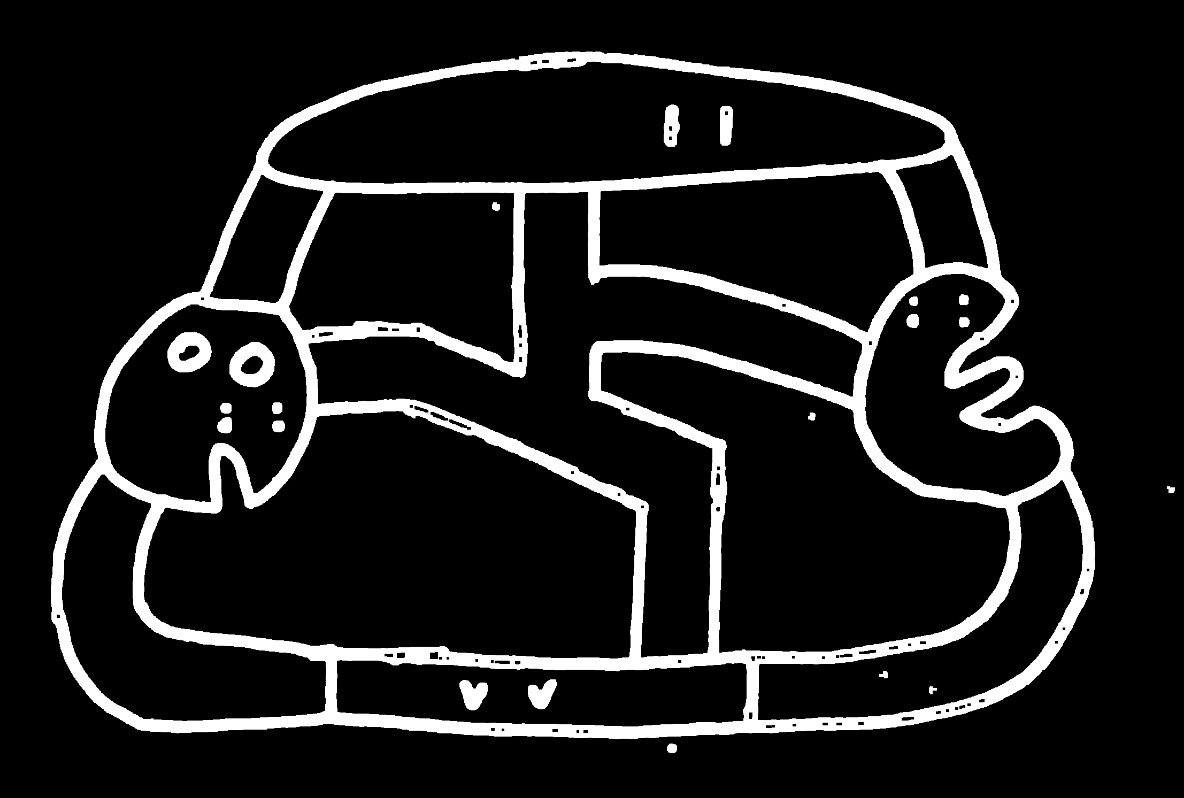
\includegraphics[width=\textwidth]{s1}
         \caption{Finding pencil}
         \label{fig:s1}
     \end{subfigure}
     \hfill
     \begin{subfigure}[b]{0.24\textwidth}
         \centering
         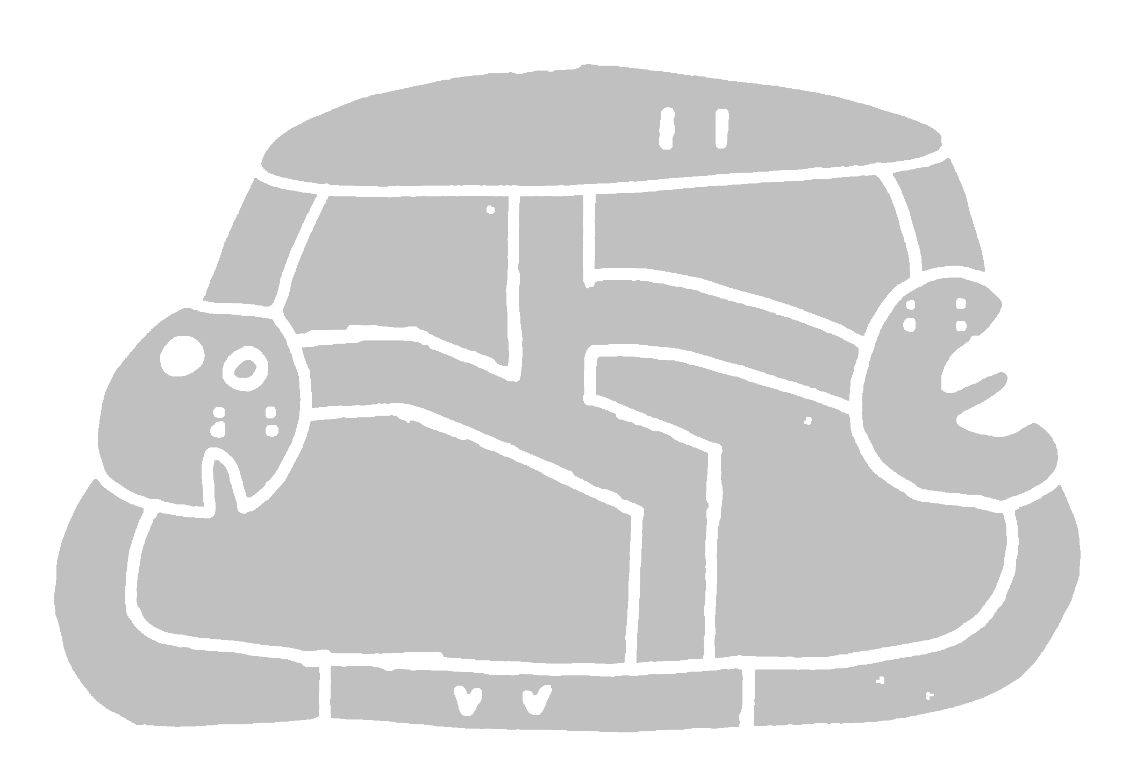
\includegraphics[width=\textwidth]{s2}
         \caption{Finding segments}
         \label{fig:s2}
     \end{subfigure}
        \caption{Segmentation}
        \label{fig:seg}
\end{figure}

\subsection{Text Recognition}
Short handwritten text is used to label segments based on what they will be in a map (floors, walls etc.). We aim to locate text precisely enough for labelling, and recognise the handwritten letters. 

The common method of detecting text with EAST and recognising text with Tesseract was tried. It was found to work best with longer words and a background without other pencil. Our application requires short labels (up to 2 letters at most) and text near other pencil, so this approach was unsuitable.

Instead convolution methods were tried. Inverted samples of handwritten letters were turned into kernels of various scales and convolved over the inverted image, with the idea being that highlights in the output showed presence of the letter. This detected well, but structural features in the sketches were also detected as text. Convolution by its definition rewards white overlap but does not reward black overlap, and does not explicitly punish opposites. For example a solid block of pencil would be detected as any sampled letter. A more specific sort of convolution is needed.

Template matching gives us the specificity needed by rewarding pixel similarity and punishing dissimilarity. Squared difference template matching was used with the sampled letters at various scales over the image, to produce a mostly whitish image with black spots where letters are found. This is inverted and thresholded so that only confident highlights are retained. These highlights from all scales are merged into one image (as a weighted average where every scale has the same weight). It was found that each true highlight tends to appear on multiple scales, so thresholding this merged image retains these and discards some random highlights. Suzuki et al. \cite{suzuki1985topological} contour finding algorithm is used to find the location of remaining highlights. As a further step of narrowing down true highlights, on the sketch we use double letters as labels (e.g. "XX"). So we look for pairs of highlights within a certain distance and angle range. The midpoint of each pair and the letter is recorded. This gives us the text label letters and locations. Figure \ref{fig:text} shows this whole process.

\begin{figure}[h]
     \centering
     \begin{subfigure}[b]{0.24\textwidth}
         \centering
         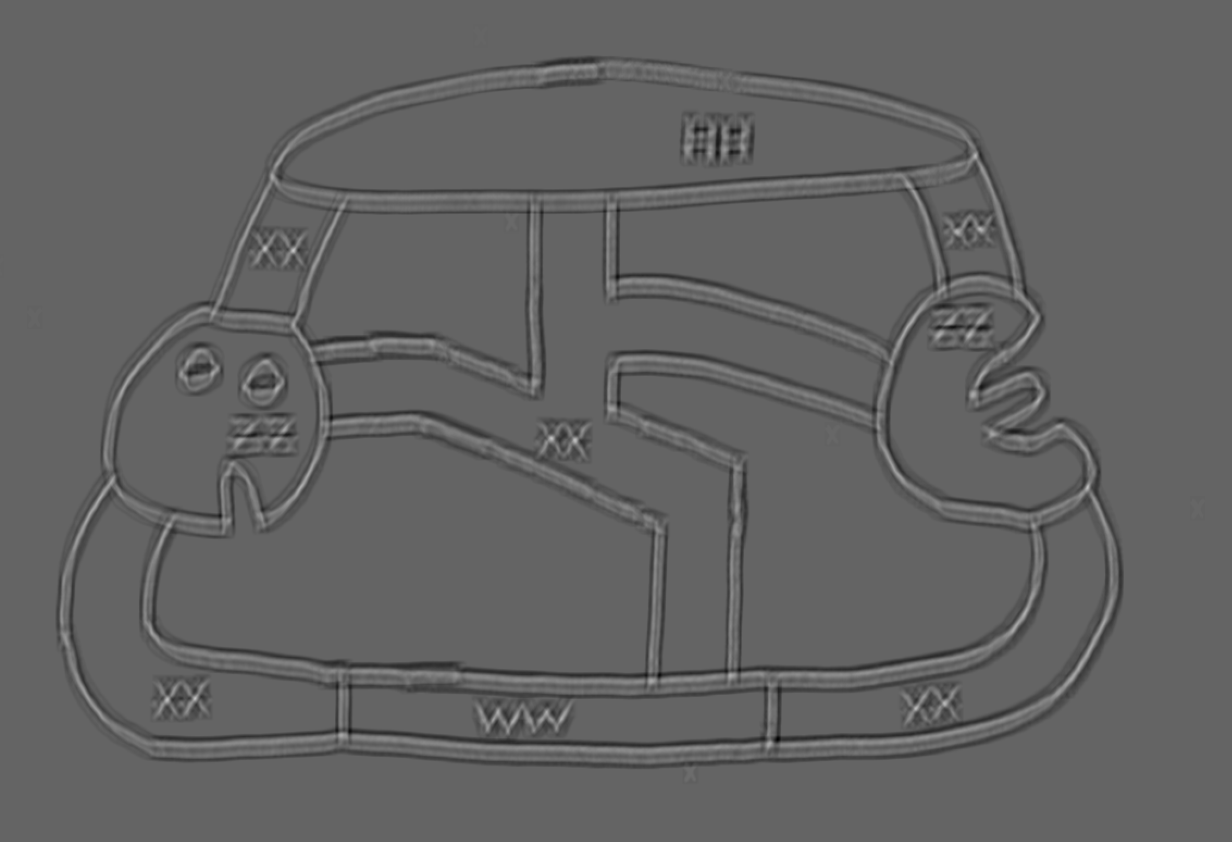
\includegraphics[width=\textwidth]{t1}
         \caption{Squared difference template match of the letter X}
         \label{fig:t1}
     \end{subfigure}
     \hfill
     \begin{subfigure}[b]{0.24\textwidth}
         \centering
         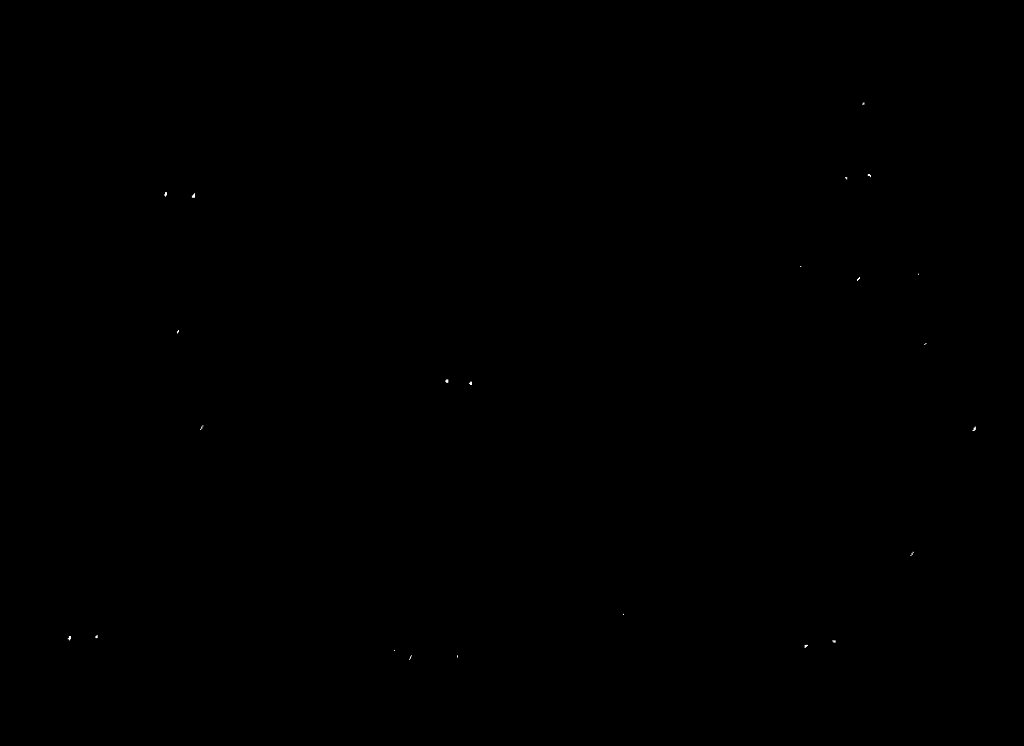
\includegraphics[width=\textwidth]{t2}
         \caption{Single scale detections (letter X)}
         \label{fig:t2}
     \end{subfigure}
     \begin{subfigure}[b]{0.24\textwidth}
         \centering
         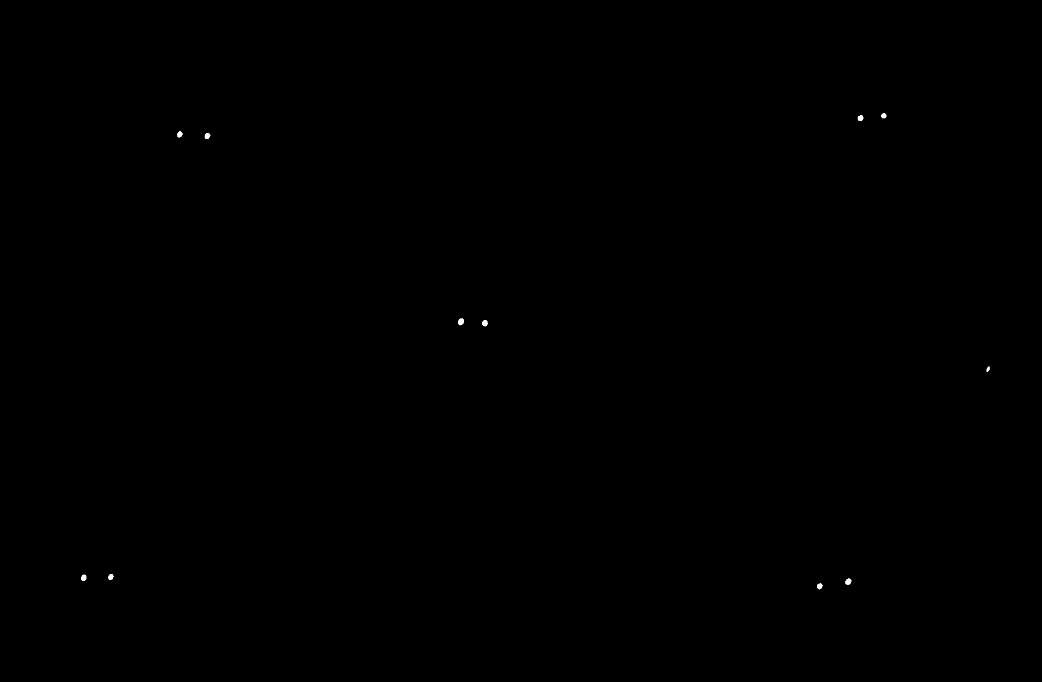
\includegraphics[width=\textwidth]{t3}
         \caption{Confidence across multiple scales (letter X)}
         \label{fig:t3}
     \end{subfigure}
     \hfill
     \begin{subfigure}[b]{0.24\textwidth}
         \centering
         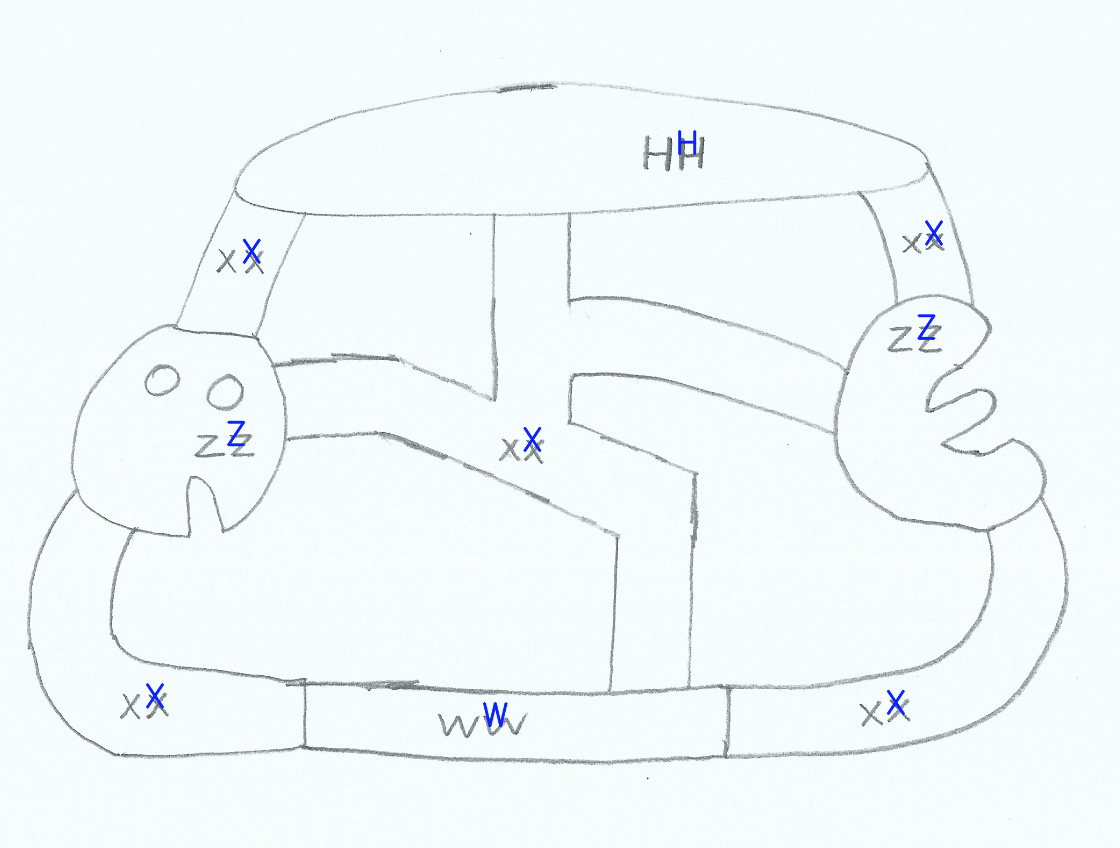
\includegraphics[width=\textwidth]{t4}
         \caption{Detected Pairs}
         \label{fig:t4}
     \end{subfigure}
        \caption{Text detection and recognition through template matching}
        \label{fig:text}
\end{figure}

\subsection{Labelling and Gap Filling}

From the segments and text labels we want to produce an image where each label has a certain colour, and each segment with that label is coloured that way. See Figure \ref{fig:labelling}.

Prior to segmentation, for each text label we fill a white rectangle over it so it isn't interpreted as a structural segment. This does not need to perfectly cover the text, but does need to reach the top and bottom of the text, so that flood filling and pencil gap filling work later.

After segmentation we colourise segments. For each text label, we use a user-defined lookup table to find its colour, then flood fill that colour from the label's location. This gives an image where labelled segments are coloured, background and pencil is white, and unlabelled segments are gray. From this point on we consider background and unlabelled segments to be "wall". We replace white and gray with black as they can be treated as the same from now on. To improve efficiency of the gap filling step we crop down the image to remove extraneous background, and scale the image down (the loss in precision is irrelevant when compared to the inaccuracy in segmentation). 

We want to fill in the black gaps left by pencil marks, both between segments (intended structural marks) and within segments (typically produced by uncovered text). For this we make PENCIL\_THICKNESS passes over the image, where PENCIL\_THICKNESS is half the width of the widest pencil mark we need to cover. In each pass if a black pixel has a coloured neighbour, it becomes that colour. This slowly grows the coloured segments until they meet each other, removing inter-segment gaps. It also fills in internal holes. After this step any remaining black segments are considered to be wall, and filled in with the "wall" colour. This gives a simplified image with colourised segments for the rest of the program to operate on. See Figure \ref{fig:labelling}.

\begin{figure}[h]
     \centering
     \begin{subfigure}[b]{0.24\textwidth}
         \centering
         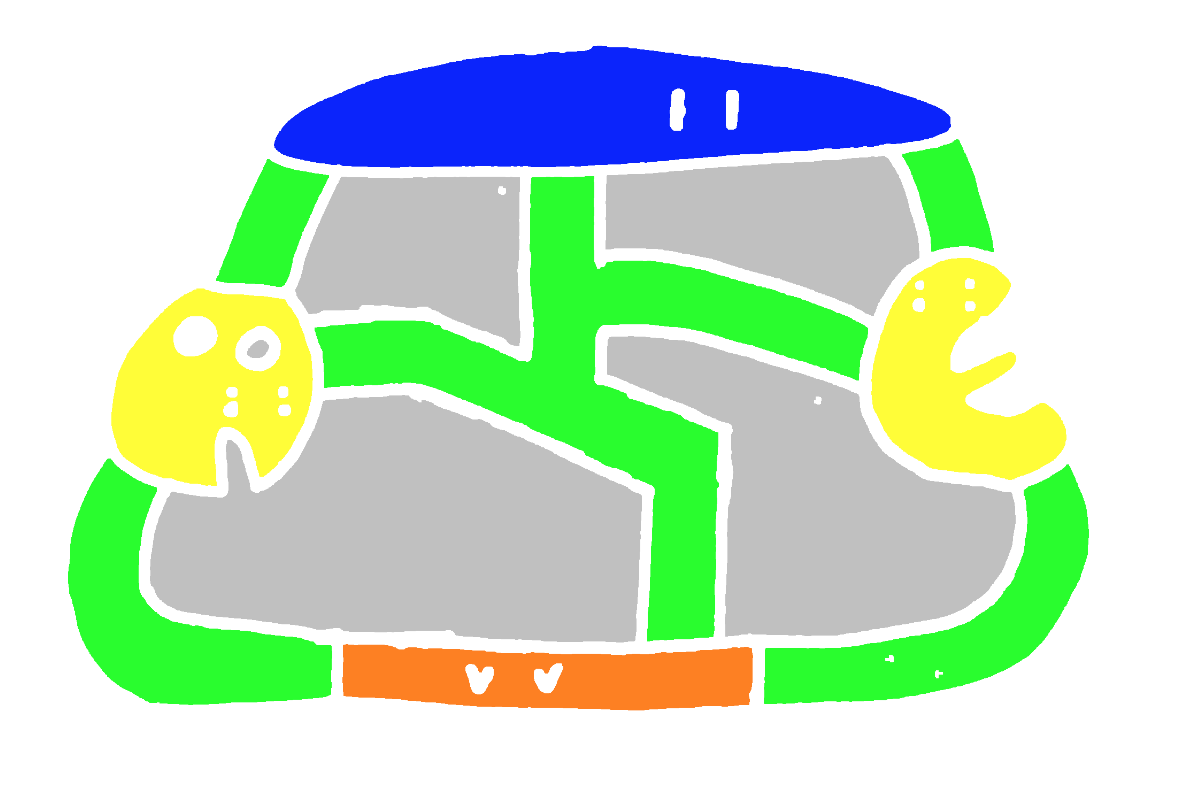
\includegraphics[width=\textwidth]{l1}
         \caption{Colouring segments using text labels}
         \label{fig:l1}
     \end{subfigure}
     \hfill
     \begin{subfigure}[b]{0.24\textwidth}
         \centering
         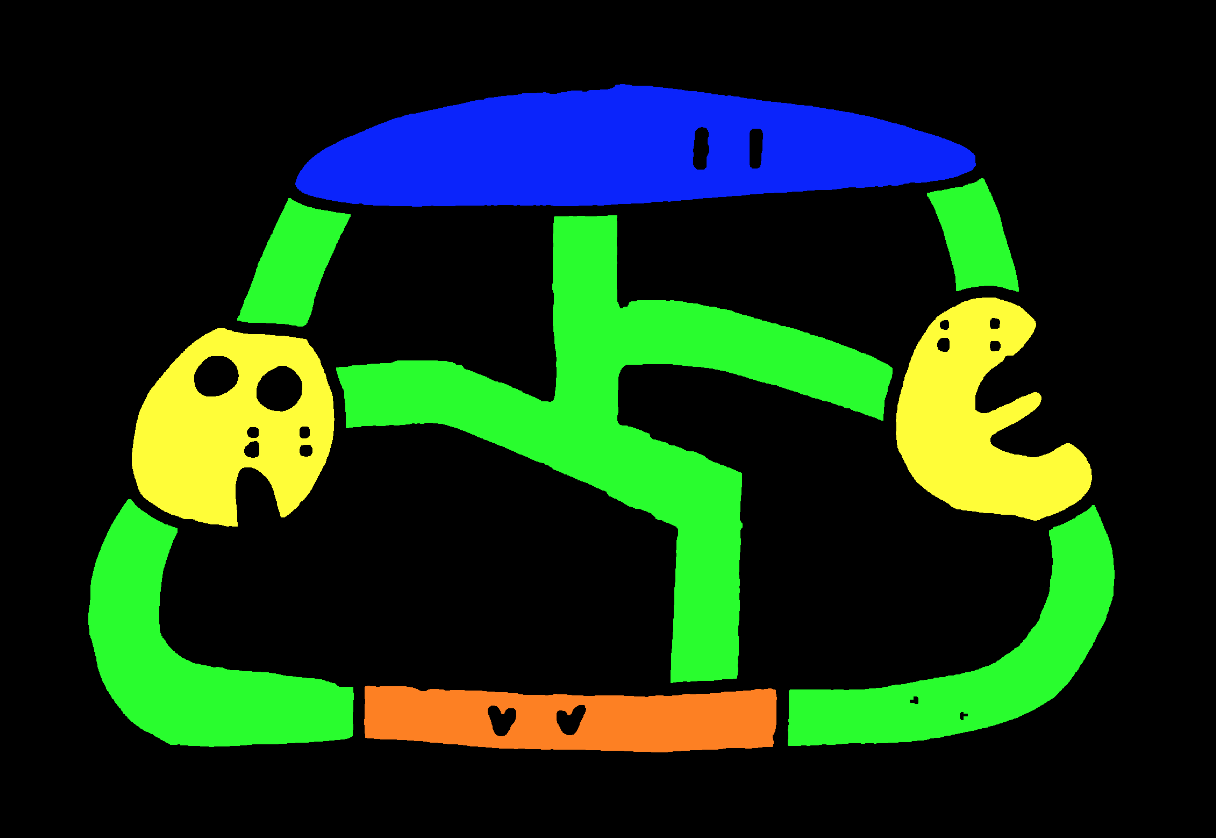
\includegraphics[width=\textwidth]{l2}
         \caption{Replacing unknown regions with black}
         \label{fig:l2}
     \end{subfigure}
     \begin{subfigure}[b]{0.24\textwidth}
         \centering
         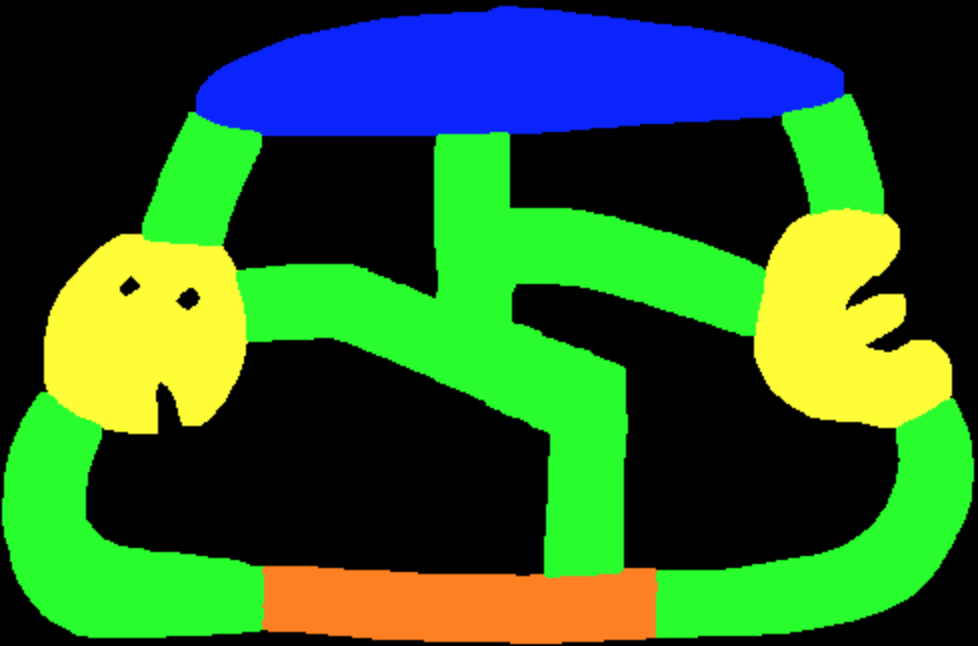
\includegraphics[width=\textwidth]{l3}
         \caption{Gap filling through dilation}
         \label{fig:l3}
     \end{subfigure}
     \hfill
     \begin{subfigure}[b]{0.24\textwidth}
         \centering
         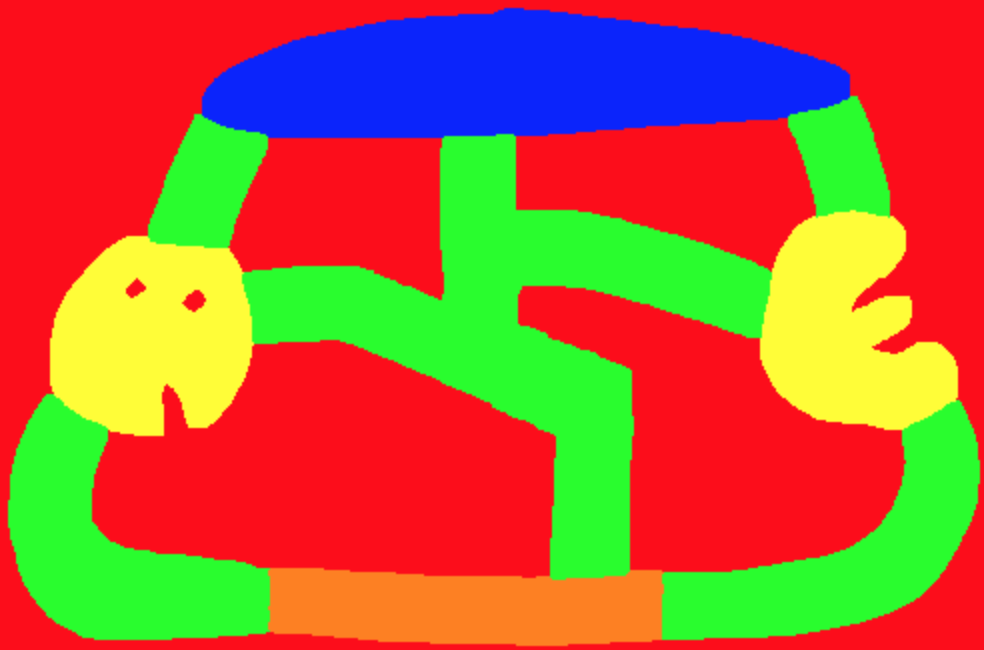
\includegraphics[width=\textwidth]{l4}
         \caption{Remaining segments coloured as wall}
         \label{fig:l4}
     \end{subfigure}
        \caption{Segment labelling and gap filling}
        \label{fig:labelling}
\end{figure}

\subsection{Segment Bordering and Triangulation}

We aim to find the border of each coloured segment, simplify it, and triangulate it to make brushes for the map file. This section operates independently of the prior sketch processing so that computer drawn images can be used.

Flood fill is used to find the pixels in each segment. A simple border walk is used to find the exact pixel by pixel border. Borders are simplified with a tolerance as a proportion of the area of the segment. Some preprocessing passes are made which operate locally, to reduce complexity. Firstly for any 3 collinear points the middle point is removed. Secondly when a corner of 1 pixel in width or height is encountered, the corner point is removed. After this tolerance based removals are applied globally, each time looking for the point which when removed changes the segment area the least. Only concavities are removed, which is suitable in this context as it ensures no gaps between the final map objects.

The colour of segments are used as labels to generate map objects. Map objects have borders and a type (wall, floor etc.). For each object its border is triangulated. This uses a fairly simple approach of cycling around the border looking for valid triangles (counter-clockwise, not intersecting the border's edges, and not containing another border point). A valid triangle is added to the result. The polygons left over from removing this triangle are themselves triangulated recursively to find the remaining triangles. 


\section{Results}

\subsection{Setup}
OS: macOS 10.13.4

Processor: 2.4 GHz dual core I5-4258U

IDE: Visual Studio Code

Language: Python 3.7.2

Device: PC

Camera: 300dpi printer scanner (Deskjet 3070 B611)

OpenCV Version: 4.5.1

\subsection{Segmentation}

Segmentation accuracy was tested with Hamming distance, comparing against a manual segmentation. In proportion to the size of the image, there was an 8.0\% difference between the algorithmic segmentation and the manual segmentation. For reference two different manual segmentations had a 2.6\% difference. We can visually inspect Figure \ref{fig:segtest} to see that the algorithmic segmentation thickens non-walls and thins walls, which accounts for the larger difference.

\begin{figure}[h]
     \centering
     \begin{subfigure}[b]{0.23\textwidth}
         \centering
         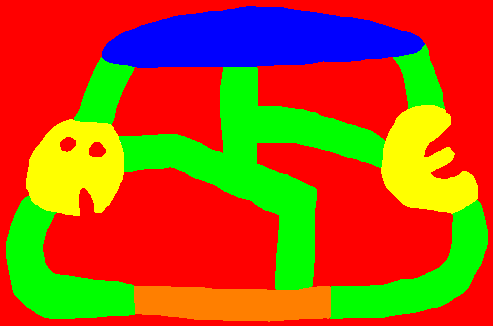
\includegraphics[width=\textwidth]{manualseg}
         \caption{Manual Segmentation}
         \label{fig:manualseg}
     \end{subfigure}
     \hfill
     \begin{subfigure}[b]{0.23\textwidth}
         \centering
         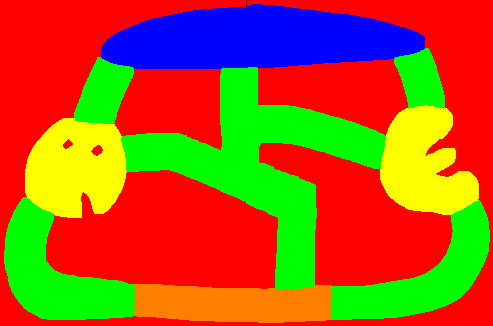
\includegraphics[width=\textwidth]{outputseg}
         \caption{Our Segmentation}
         \label{fig:outputseg}
     \end{subfigure}
        \caption{Segmentation comparison}
        \label{fig:segtest}
\end{figure}

A better solution would treat the pencil filling stage as a closing operation rather than just a dilation.

\subsection{Text Recognition}

The commonly described EAST + Tesseract method detects 90\% of double characters but only recognises 30\% of them due to its dependency on recognising complete words. Our method using sample template matching detects and recognises 100\% of double characters, with no false detections on other lines. For a comparison see Figure \ref{fig:texttest}.

\begin{figure}[h]
     \centering
     \begin{subfigure}[b]{0.4\textwidth}
         \centering
         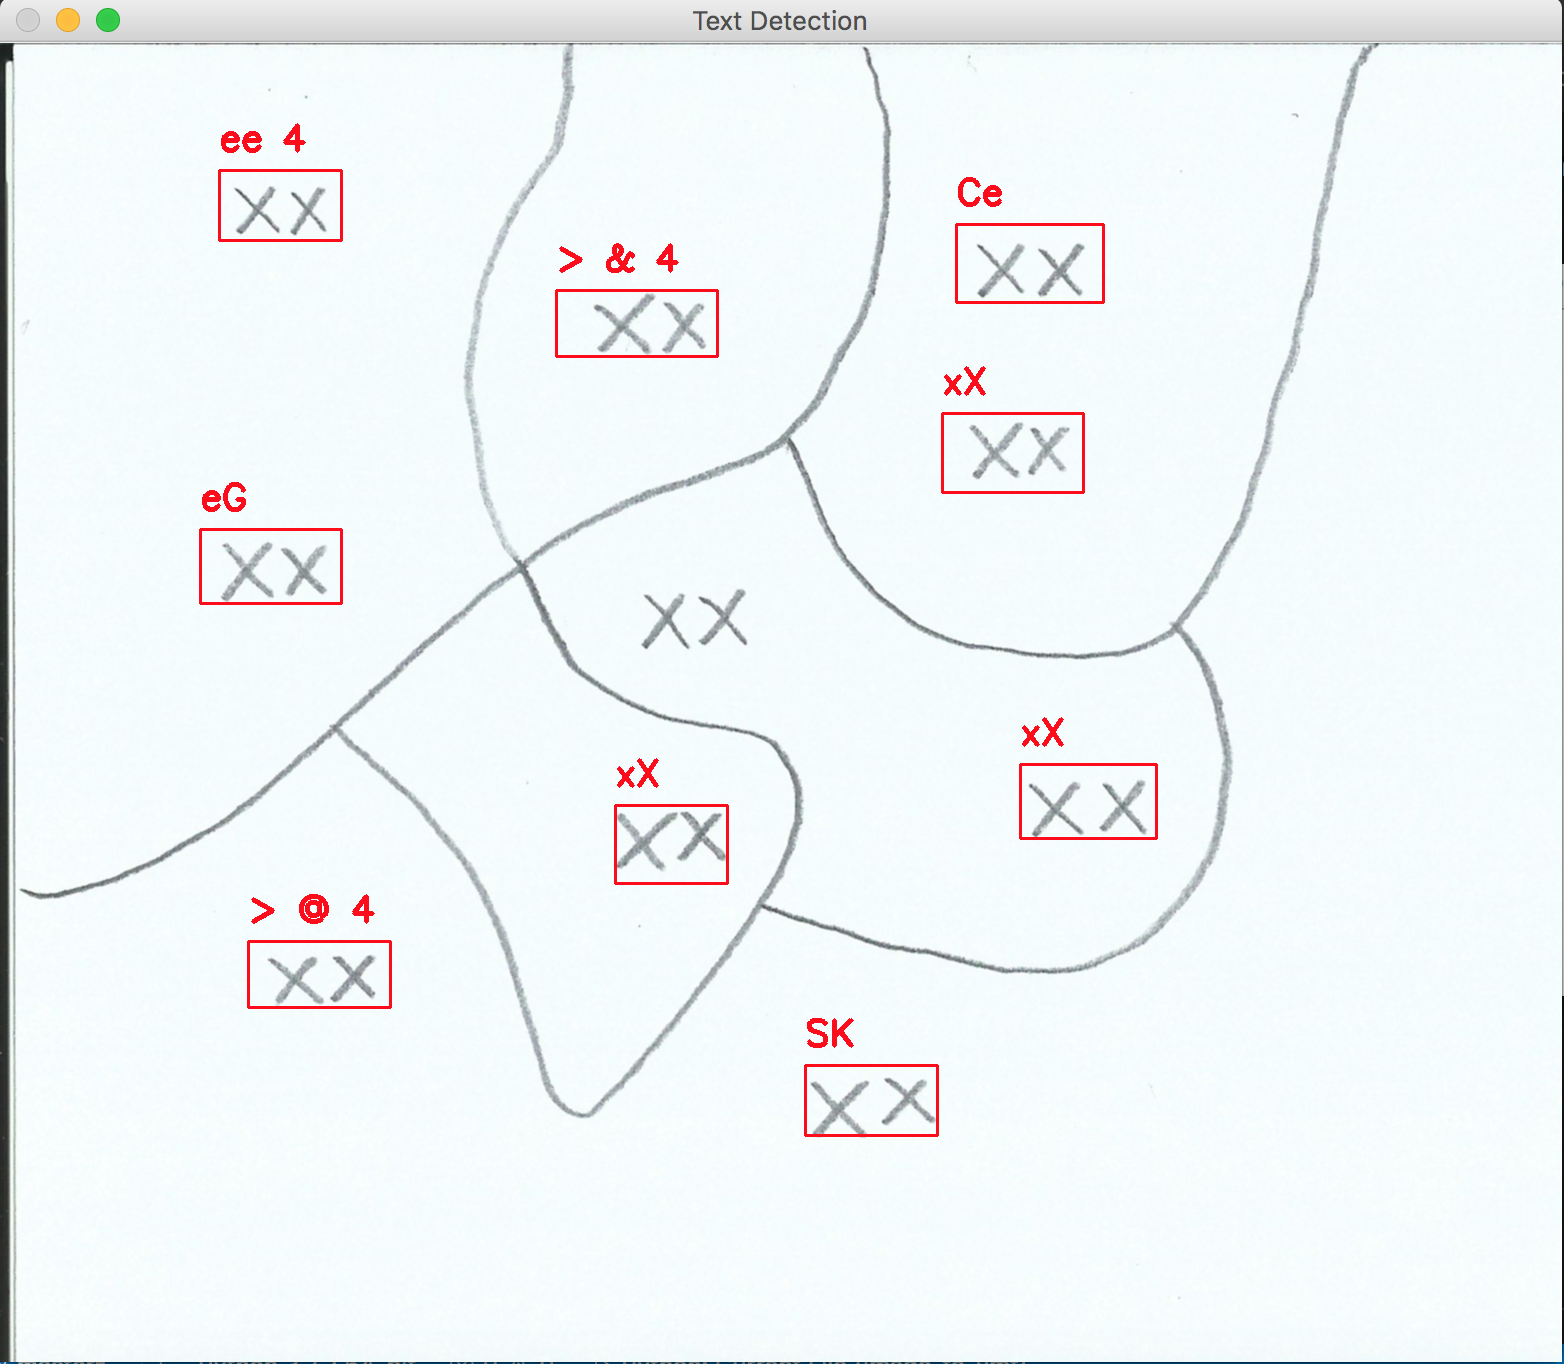
\includegraphics[width=\textwidth]{ocrprior}
         \caption{Common OCR Method}
         \label{fig:ocrprior}
     \end{subfigure}
     \hfill
     \begin{subfigure}[b]{0.4\textwidth}
         \centering
         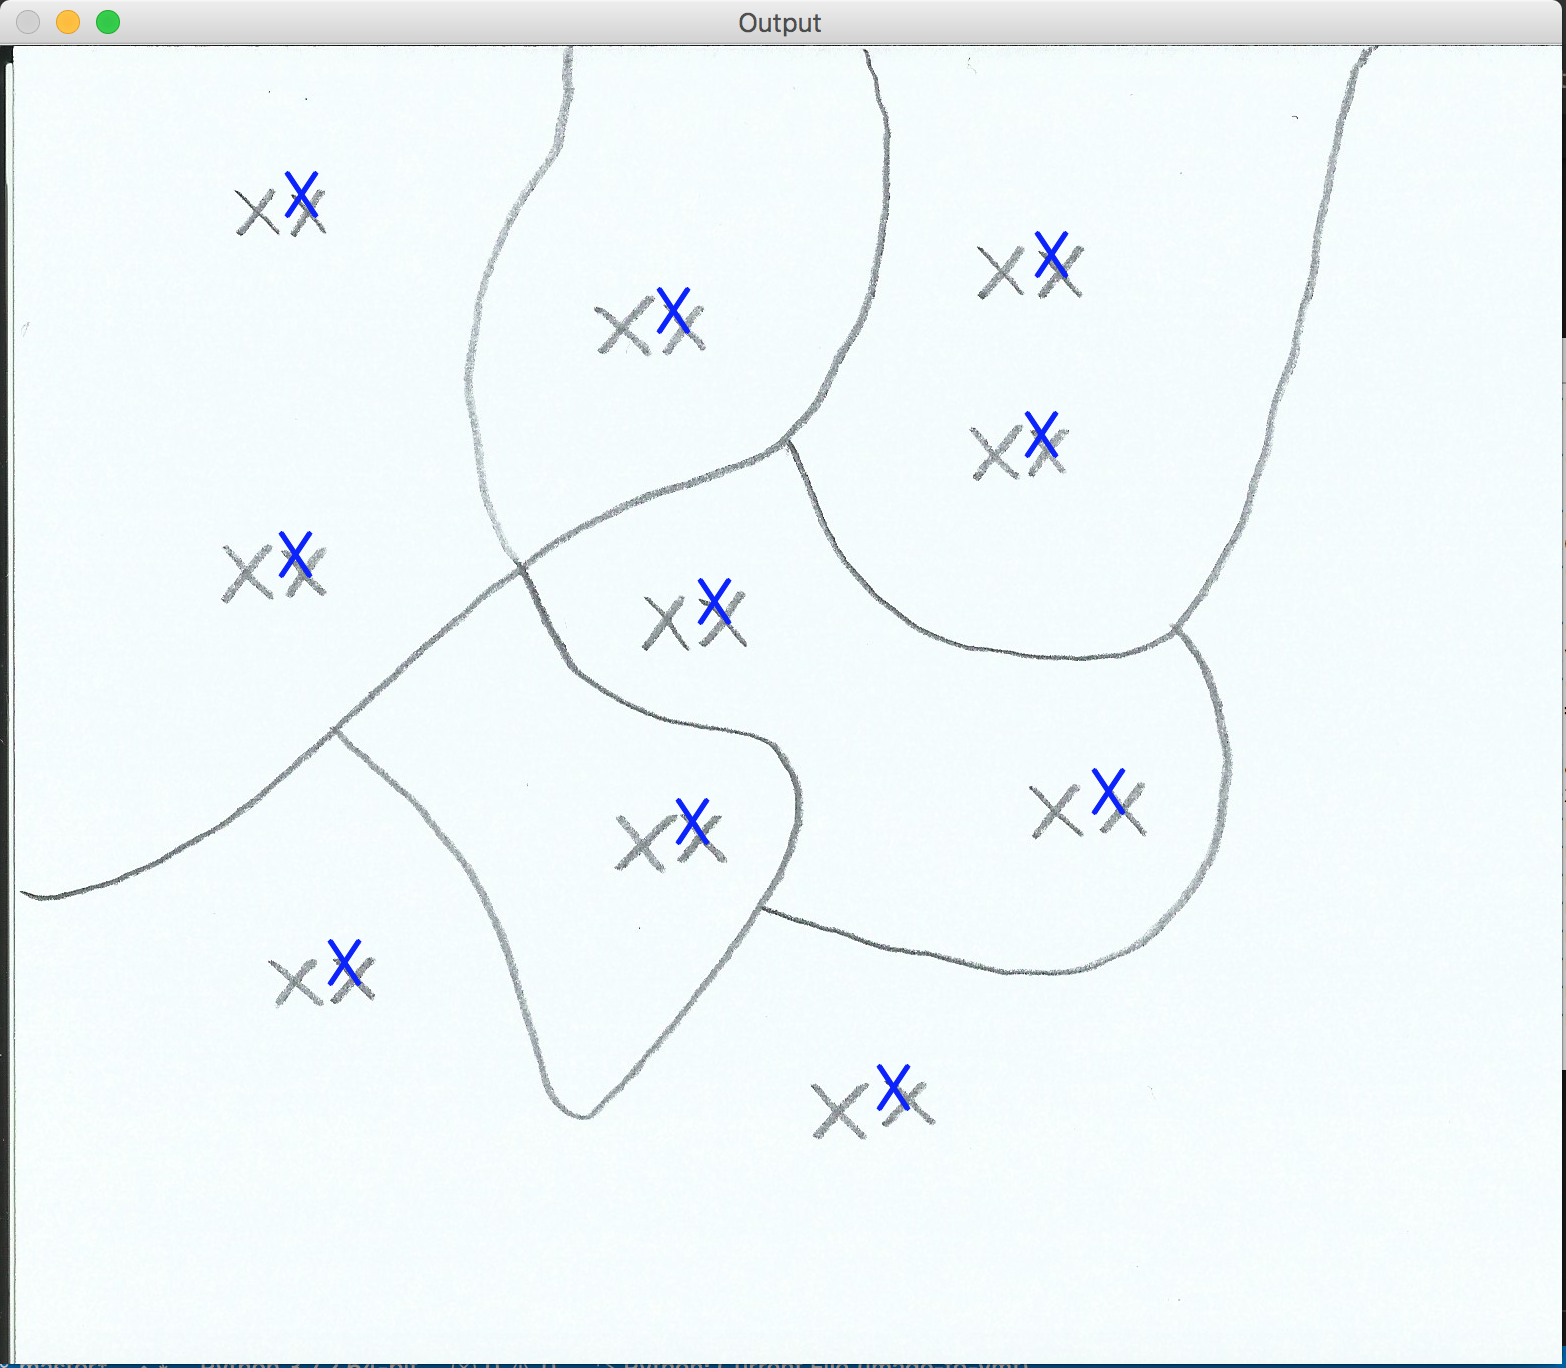
\includegraphics[width=\textwidth]{textrec}
         \caption{Our Sample Recognition}
         \label{fig:textrec}
     \end{subfigure}
        \caption{Text detection and recognition}
        \label{fig:texttest}
\end{figure}

On the sample image in Figure \ref{fig:texttest} the EAST + Tesseract method takes just 5 seconds to complete, whereas our method takes 43 seconds. For an image $W*H$, template symbols $M*N$, and number of template rescalings $X*Y$, our method has complexity $O(W*H*M*N*X*Y)$. On A4 pages at 300 ppi, our method takes about 3-4 minutes for text recognition. Template size isn't feasible to adjust, however image size and template rescalings are. Image size can be adjusted by manual cropping after scanning. Number of template rescalings can be reduced by consistently drawing letters at similar sizes, and setting tighter bounds on their possible size.

\bibliographystyle{IEEEtran}
\bibliography{references}

\end{document}